\chapter{图的对象与表示}
\label{chap:graph-objects}

四个二值变量$z_i\in\{0,1\}$，$i\in V=\{1,2,3,4\}$，要同时满足三条局部规则：
$z_1,z_2$恰有一个取$1$；$z_3=1$时必须有$z_1=1$；
$z_4=1$时，$z_2,z_3$至少有一个取$1$。
这三条规则分别只涉及$\{1,2\}$、$\{1,3\}$和$\{2,3,4\}$中的变量，
没有哪一条需要同时读入全部四个变量。
要利用这种局部性，先得把“哪些变量直接出现在同一条规则中”记录下来：
把共同出现的每一对变量连接起来，得到边集
\begin{equation}
  E=\bigl\{\{1,2\},\{1,3\},\{2,3\},\{2,4\},\{3,4\}\bigr\}.
  \label{eq:graph-theory-running-edges}
\end{equation}
这就得到一张图，如图~\ref{fig:graph-theory-running-graph}：左右两个三角形共享顶点$2,3$。

\begin{figure}[htbp]
  \centering
  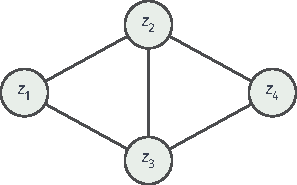
\includegraphics[width=50.281mm]{figures/01-mathematical-preliminaries-upper/03-graphs-and-signals/tikz/graph-theory-running-graph/figure.pdf}
  \caption{由四变量约束的作用域导出的关系图。边表示两个变量共同出现在至少一个
  约束中；共享顶点集合$\{2,3\}$连接左右两侧。图没有记录约束的具体真值表，
  也没有预先指定边长、容量或相似度。}
  \label{fig:graph-theory-running-graph}
\end{figure}

为什么不直接用向量或矩阵记录这些关系？上一部分的信号总有规则的位置索引，
相邻项就是相邻时刻；矩阵则预设“行对象与列对象两两配对”。
这里的关系是稀疏且不规则的：一个变量可能只与两个同现，另一个却与五个相连，
关系也未必成对出现。用完整矩阵记录，会为大量并不存在的关系预留位置，
更看不出“沿关系能否从一处走到另一处”。因此需要一种只保留
“哪些个体直接相关”的对象，这就是图。

但图有意只记录最少的信息。它只记录哪些个体直接相关，
不记录相关有多强、是什么性质；边表示两个变量共同出现，
却没有保存规则的真值表——三条两两连接并不会把三元规则变成三个等价的二元约束。
边长、容量、相似度、方向和局部函数都要另外补上。
正因为不预设关系的含义，同一种图结构才能同时承担不同任务：
在样本之间表示相似，在变量之间表示统计依赖，在任务之间表示先后次序。

同一条边上附的数字，在不同任务里读法完全不同。
本章先回答“一条边到底保存了什么”：先确定顶点、边、方向与数值属性，
再区分二元关系与高阶关系，然后给出便于计算机使用的矩阵表示，
并顺带建立沿边差分、拉普拉斯与能量这套后两章反复调用的公共算子，
最后说明顶点换名时哪些信息应当保持不变。
固定共享变量$\{2,3\}$以后，左右两侧的局部计算可以分别进行，
这张贯穿图会在本章和后续各章反复出现。

\section{二元关系的图表示}
\label{sec:graph-theory-binary-relations}

本节先确定最基本的图：哪些点、哪些点之间有连接、连接是否带方向，
以及连接上附的数值表示什么。这些属性可以组合——
有向与无向描述方向，加权与无权描述是否附带数值，
并不是几个互斥的图类别。

\subsection{顶点、边与方向}

把每个变量记为一个顶点，把共同出现在一条规则中的一对变量连成边，
边记录的就是直接关系；经过其他变量才能建立的联系暂时不计入。

\paragraph{无向图}
\term{无向图}（undirected graph）写作$\mathcal G=(V,E)$，其中$V$是有限顶点集合，
$E$是由不同顶点的无序对组成的边集合。本章默认不考虑自环（一个顶点连到自身），
也不考虑同一对顶点之间的平行边；若要允许它们，就得另外保存边的身份或重数，
不能继续把边集当成普通无序对集合。若$\{i,j\}\in E$，称$i,j$相邻，二者互为邻居。

\paragraph{邻域}
顶点$i$的\term{邻域}（neighborhood）是它的全部邻居：
\[
  N(i)=\{j\in V:\{i,j\}\in E\}.
\]
在贯穿图中可以逐条读出$N(2)=\{1,3,4\}$、$N(1)=\{2,3\}$。
“枚举$i$的邻居”输出的正是这样一份点的列表，它是后面遍历与邻接访问共用的接口。

\paragraph{顶点的度}
邻域的大小称为顶点$i$的（无权）\term{度}（degree）：
\[
  d_i=|N(i)|.
\]
贯穿图中$d_2=3$、$d_1=2$。度只统计直接邻居的个数，
不统计沿边经过若干步才能到达的顶点；后者要到下一章讨论路径时才计算。
带权时另有“\term{加权度}”，那是把邻边权重累加起来，放在本章拉普拉斯一节定义，
不要与这里的邻居数混为一谈。

\paragraph{有向图与弧}
当关系具有方向——“$i$依赖$j$”与“$j$依赖$i$”是两条相反的信息，
任务依赖、概率生成和网页链接都天然不对称——无序对就不够用了。
\term{有向图}（directed graph）写作$\mathcal G=(V,A)$，
其中$A\subseteq V\times V$是有序对（弧）的集合，仍排除$(i,i)$。
弧$(i,j)$记作$i\to j$，表示允许从$i$一步到$j$；它并不自动包含反向弧$j\to i$。
后续矩阵编码统一采用“行是起点、列是终点”的约定。

\paragraph{入邻域与出邻域}
对顶点$j$，指向它的顶点组成入邻域，由它指出去的顶点组成出邻域：
\[
  N^-(j)=\{i:i\to j\},\qquad N^+(j)=\{i:j\to i\}.
\]
二者的大小分别称为\term{入度}（in-degree）与\term{出度}（out-degree）。
它们沿相反方向读取同一条弧，所以报告“邻居”时必须说明是哪一种。
有向图中常把入邻居称为父节点、出邻居称为子节点，
但这只是方向上的称谓；箭头本身不提供因果解释，
本章只使用连接与方向，其概率与生成机制含义留待相应卷册。

\subsection{边的数值与结构}

结构边只说明两点相邻。同一条边上还可以附一个数值，
这个数值在不同任务里代表完全不同的量，算法入口必须先声明它的语义和取值条件。

\paragraph{边长}
把数值解释为长度或成本$\ell_{i,j}$时，它将在沿路线行走时逐条相加，
累计成本越小越有利。这个数不必等于画图时线段的几何长度；
零长度也可能表示一条可以免费通行的结构边。

\paragraph{边容量}
把数值解释为容量$c_{i,j}$时，它限制允许通过这条通道的流量上界。
容量越大，限制越宽松；零容量表示该通道不能输送正流量。
容量不应当作路径成本直接相加，它回答的是“最多能过多少”，不是“经过要付多少”。

\paragraph{相似度权重}
把数值解释为两点的相似程度$w_{i,j}$时，在后面的平滑与划分中，
大权重通常更强地惩罚两端取值的差异。无向权重满足$w_{i,j}=w_{j,i}$，
有向权重则不必对称。

\paragraph{零权边}
由此可见，零值的含义由当前任务决定：免费道路、零容量通道和零相似度是三回事。
无论哪种，零数值都不自动删除结构边。“能否走到”查的是边集，与权重是否为零无关；
线性加权汇总查的才是作用权重。必要时两者要分别保存。

\paragraph{\term{正权支撑}图}
对有限无向非负权图，把真正起作用的边收集起来：
\[
  E_+=\bigl\{\{i,j\}\in E:w_{i,j}>0\bigr\},
\]
称$(V,E_+)$为正权支撑图。后面的拉普拉斯、谱与扩散只受$E_+$中的权重影响，
因为零权边在差分与平均中贡献为零；而长度问题是否允许使用零权边，
仍按该问题自己的规则判断，不能一概而论。

\subsection{限制顶点集与诱导子图}

只研究一部分对象时，不能悄悄改掉它们之间的关系。
给定顶点子集$U\subseteq V$，保留$U$中的顶点，并保留原图中
两端都属于$U$的全部边（有向图则保留两端都在$U$中的全部弧），
得到的图称为$U$上的\term{诱导子图}（induced subgraph），记作$\mathcal G[U]$。

在贯穿图中取$U=\{1,2,3\}$，诱导子图必须保留$\{1,2\},\{1,3\},\{2,3\}$三条边；
若只留下$1-2-3$这两条边，虽然仍是一个子图，却漏掉了边$\{1,3\}$，
因而不是该顶点集上的诱导子图。诱导子图这一操作后面会反复出现：
取祖先图、删除分隔集后的余图、分块时的局部块，本质上都是在某个顶点集上取诱导子图。

\section{高阶关系的因子表示}
\label{sec:graph-theory-higher-order-scopes}

二元关系只能说“哪两个变量同现”。但“$z_4=1$时，$z_2,z_3$至少有一个取$1$”
是一条同时约束三个变量的规则。把它改画成$2$—$3$、$3$—$4$、$2$—$4$三条边，
虽然保留了哪些变量同现，却丢掉了“这三个变量进入同一条规则”的信息。
本节区分“哪些变量共同出现”与“这些变量的哪些取值被允许”，
并为这种高阶规则保留身份。

\subsection{局部函数与作用域}

\paragraph{局部配置与局部函数}
先固定$z_2,z_3,z_4$各自的取值集合（这里都是$\{0,1\}$），
它们的一次联合取值$(z_2,z_3,z_4)$称为一个局部配置。
上述规则可以写成一个$0/1$指示函数
\[
  \phi_{2,3,4}(z_2,z_3,z_4)=
  \begin{cases}
    0,&(z_2,z_3,z_4)=(0,0,1),\\
    1,&\text{其他二值输入}.
  \end{cases}
\]
它读入三个变量的一次赋值，输出该赋值是否满足规则。
这样定义在少数几个变量上、给出成本、权重或可行性的函数，称为局部函数或因子（factor）。

\paragraph{作用域}
一个局部函数需要读取哪些变量，由这些变量的下标集合记录，称为它的作用域（scope）。
这里$\phi_{2,3,4}$的作用域是$\{2,3,4\}$。作用域保存的是输入位置，不保存函数真值表；
同一个作用域上完全可以附不同的函数。因此“知道作用域”与“知道规则内容”是两回事，
记录同现关系并不等于给出了函数的分解。

\subsection{作用域的三种表示}

\paragraph{超边与超图}
要保留“若干变量属于同一个作用域”，最直接的做法是允许一条边包含多个顶点：
每条超边是一个顶点子集，不限于两个顶点，由此得到\term{超图}（hypergraph）。
超边$\{2,3,4\}$在此记录三元作用域；它仍然不保存局部函数的具体取值。

\paragraph{因子图与二部图}
另一种做法把变量和局部函数分成两组节点，只在变量属于某函数作用域时连边。
两组节点内部都没有边的图称为\term{二部图}（bipartite graph）；
按这种方式得到的因子图（factor graph）通常用方形节点表示因子、圆形节点表示变量，
既保留了因子的身份，又标明了每个因子读哪些变量。完整求值仍需另外保存该因子的函数表。

\paragraph{原始关系图}
若不保留因子节点，只把每个作用域内的变量两两相连，
就得到\term{原始关系图}（primal graph），简称原始图。
章首的贯穿图正是按这条规则由三条局部条件得到的：三元作用域$\{2,3,4\}$
贡献了$\{2,3\},\{2,4\},\{3,4\}$三条边。

\paragraph{成对投影的信息损失}
关键问题是：仅靠原始图上的两两关系，能不能恢复原来的高阶约束？一般不能。
考虑三元二值约束“恰有偶数个变量等于$1$”，它允许
$(000,011,101,110)$四种配置。把它投影到每一对变量上，
每一对的四种取值$(00,01,10,11)$都会在某个允许配置中出现，
于是只保留这三个成对允许关系，将不再排除任何配置，连$(001)$也被错误地放行了。

\begin{figure}[htbp]
  \centering
  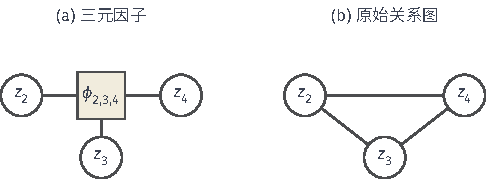
\includegraphics[width=82.282mm]{figures/01-mathematical-preliminaries-upper/03-graphs-and-signals/tikz/graph-theory-factor-scope/figure.pdf}
  \caption{三元因子与原始关系图。左侧方框是同一个依赖$z_2,z_3,z_4$的函数，
  连线表示作用域归属；右侧只保留变量共同出现的两两关系。右侧三条边不是把三元
  函数分解成三个二元函数的等价变换，也不能恢复原函数的数值。}
  \label{fig:graph-theory-factor-scope}
\end{figure}

如图~\ref{fig:graph-theory-factor-scope}所示，一个三元因子和三个二元因子
可以产生同一个三角形原始图，但前者能表达的约束未必能写成后者同时成立的形式。
因此后续的树分解与变量消元都必须保留完整作用域，不能把原始图当作原约束表。

\section{图的矩阵表示}
\label{sec:graph-theory-matrix-representations}

对象确定之后，还要选一种让计算机能高效使用的表示。
同一种连接结构要支撑性质不同的高频访问：遍历要取出某个顶点的全部邻居，
数值传播要把邻居的值按权重加起来，计算边差则要逐条取出一条边的两端。
本节先比较几种存储结构，再由邻接矩阵和关联矩阵建立邻居汇总与边差，
最后把边差汇总成贯穿全书的拉普拉斯算子及其归一化形式。

\subsection{邻接访问与存储}

\paragraph{邻接表}
遍历要反复枚举一个顶点的全部邻居。\term{邻接表}为每个顶点保存它的邻居及所需边属性。
记$n=|V|$、无向边数$m=|E|$（有向图记弧数$a=|A|$），总存储为$O(n+m)$；
无向边在两个端点各存一次，反向弧表的存储也要计入。

\paragraph{边表}
当算法需要逐条处理边（排序边、扫描边、维护残量配对）时，
\term{边表}直接保存每条边的两个端点、身份与属性。邻接表与边表可以同时使用，
多出的$O(m)$个记录应计入存储代价。

\paragraph{稠密矩阵与稀疏矩阵}
稠密矩阵为每一对顶点都预留位置，占$O(n^2)$存储；稀疏矩阵只保存实际非零条目。
分析算法代价时必须声明采用哪种表示：邻接表上沿邻居的线性遍历，
不能直接套到逐行扫描稠密矩阵上。

\paragraph{邻接矩阵}
固定顶点次序$1,\ldots,n$，\term{邻接矩阵}（adjacency matrix）
$\bm A\in\mathbb R^{n\times n}$的条目为
\[
  a_{i,j}=
  \begin{cases}
    w_{i,j},&\{i,j\}\in E\ \text{或}\ (i,j)\in A,\\
    0,&\text{其他情形},
  \end{cases}
\]
无权边取权重$1$。贯穿图对应
\begin{equation}
  \bm A=
  \begin{bmatrix}
    0&1&1&0\\
    1&0&1&1\\
    1&1&0&1\\
    0&1&1&0
  \end{bmatrix}.
  \label{eq:graph-theory-running-adjacency}
\end{equation}

\paragraph{矩阵乘法的方向}
有向情形按“行起点、列终点”约定：
\[
  (\bm A\bm f)_i=\sum_j a_{i,j}f_j
\]
读出的是顶点$i$的出邻居值之和；$\bm A^\top\bm f$则把每个起点的值沿出弧发送到终点。
图~\ref{fig:vol1-add-graph-adjacency-orientation}用只有两条弧$1\to2,1\to3$、
$\bm f=(1,2,3)^\top$的小图分别算出$\bm A\bm f=(5,0,0)^\top$（顶点$1$读取$2+3$）
和$\bm A^\top\bm f=(0,1,1)^\top$（把$f_1=1$送到两个终点）。
无向图中$\bm A$对称，两种读法才重合。
\begin{figure}[!htb]
  \centering
  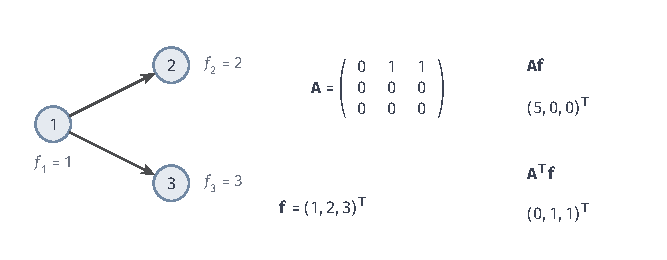
\includegraphics[width=112mm]{figures/01-mathematical-preliminaries-upper/03-graphs-and-signals/tikz/comprehension-additions/graph-adjacency-orientation.pdf}
  \caption{只有两条单位权弧$1\to2$和$1\to3$的有向图，顶点值为$\bm f=(1,2,3)^\top$。
  邻接矩阵按“行起点、列终点”存储：$\bm A\bm f$在顶点$1$处读取$2+3=5$；
  $\bm A^\top\bm f$则将$f_1=1$沿两条弧发送，顶点$2,3$各收到$1$。
  矩阵转置改变汇总方向，未改变图中弧的定义。}
  \label{fig:vol1-add-graph-adjacency-orientation}
\end{figure}
在贯穿图上取$\bm f=(1,2,3,4)^\top$，可复算$\bm A\bm f=(5,8,7,5)^\top$。
这是顶点值的线性汇总，不等于在全部变量配置上求和，后者还需要明确局部因子。

\paragraph{结构掩码}
允许零权边时，数值$0$无法区分“无边”与“零权边”。
为此另存一个结构掩码$\bm M\in\{0,1\}^{n\times n}$：存在结构边或弧时$m_{i,j}=1$，否则为$0$。
后续算法要说明自己读的是数值矩阵还是结构掩码；例如两顶点空图与两顶点零权单边图
都可能有$\bm A=\bm 0$，连接关系却不同。

\subsection{关联矩阵与边差}

\paragraph{关联矩阵}
要计算每条边两端的差，给每条无向边任选一个临时方向，构造\term{关联矩阵}
（incidence matrix）$\bm B\in\mathbb R^{n\times m}$：
边$e$从$i$指向$j$时，对应列在$i$处取$1$、在$j$处取$-1$，其余为零。
于是
\[
  (\bm B^\top\bm f)_e=f_i-f_j
\]
正好是该边两端的差。临时方向只用于统一记录这个差值。

\paragraph{边差的加权汇总}
令$\bm W_E=\operatorname{diag}(w_e:e\in E)$为边权对角矩阵，则
$\bm B\bm W_E\bm B^\top$分三步完成“取边差—按边权缩放—汇总回顶点”。
若反转某些边的临时方向，相当于右乘一个对角元为$\pm1$的符号矩阵$\bm R$
（反向的边取$-1$，其余取$1$）：$\bm B'=\bm B\bm R$。
由于$\bm R\bm W_E\bm R=\bm W_E$，所得无向加权算子并不随临时方向改变。
这一便利只属于无向边的临时定向，不能用来消除真正有向图中的方向。

\subsection{组合拉普拉斯与沿边变化}

下面把边差汇总成一个算子。这套算子是第14章图划分与第15章谱方法、扩散共用的基础，
因此在此一次性建立；如何用它做离散优化、如何按谱滤波，则分别留给那两章。

\paragraph{加权度}
固定有限无向、权重非负的图。顶点$i$的加权度及其对角矩阵为
\[
  d_i^{(w)}=\sum_j w_{i,j},\qquad
  \bm D^{(w)}=\operatorname{diag}(d_1^{(w)},\ldots,d_n^{(w)}).
\]
无权度$d_i$数的是邻居个数，加权度$d_i^{(w)}$累计的是相邻边的作用强度；
只有每条结构边权均为$1$时二者才相同。

\paragraph{组合拉普拉斯}
\term{组合图拉普拉斯}（combinatorial graph Laplacian）定义为
\begin{equation}
  \bm L=\bm D^{(w)}-\bm W=\bm B\bm W_E\bm B^\top,
  \label{eq:graph-theory-combinatorial-laplacian}
\end{equation}
其逐点作用为
\[
  (\bm L\bm f)_i=\sum_j w_{i,j}(f_i-f_j).
\]
它把本点值与各邻居值之差按权重汇总；相邻值已经相等的边不再贡献。
每条边给两端对角元各加$w_e$、给两个交叉位置各加$-w_e$，合计正是$\bm D^{(w)}-\bm W$。
常数向量满足$\bm L\bm 1=\bm 0$，因为常数在每条边上都没有差异。

\paragraph{沿边变化能量}
拉普拉斯对应的二次型把全部边差平方按权重累加起来：
\begin{equation}
  \bm f^\top\bm L\bm f
  =\sum_{\{i,j\}\in E}w_{i,j}(f_i-f_j)^2
  =\frac12\sum_{i,j}w_{i,j}(f_i-f_j)^2.
  \label{eq:graph-theory-dirichlet-energy}
\end{equation}
两种写法只是计数方式不同：按无向边$\{i,j\}$求和每条边计一次，无需系数；
按有序对$(i,j)$求和每条边计两次，因此乘$1/2$。
因为权重非负、每项是平方，这个量恒非负，所以$\bm L$对称半正定。
若边权允许为负，非负性便不再成立；真正的有向图也另有不同的拉普拉斯，
不能直接套用这里的对称谱结论。

\paragraph{零能量的逐边条件}
二次型为零，当且仅当每一个平方项都为零，即每条正权边的两端值相等：
\[
  \bm L\bm f=\bm 0
  \quad\Longleftrightarrow\quad
  f_i=f_j\ \text{对所有}\ \{i,j\}\in E_+.
\]
零权结构边不强制两端相等。例如一条结构边仍在但权为$0$，
它两端取不同值也不会使能量变大。至于“沿正权边把相等关系传遍一个连通分量、
从而零空间由各分量常数组成”这一完整刻画，要用到下一章才正式建立的路径与连通分量，
因此放在第15章谱方法入口完成；这里只确定逐边条件本身。

\subsection{归一化算子与度量}

组合拉普拉斯直接比较顶点值。但同样的端点差，在连接很多的顶点上会被累计更多次；
有时希望把连接总量也计入顶点幅度的衡量。这就需要归一化。
本节的共同前提是无向、非负权重；零度顶点要单独约定。
本节起$d_i$一律是加权度$d_i^{(w)}$的简写，不再表示邻居数。

\subsubsection{对称归一化拉普拉斯}

\paragraph{度加权内积与坐标缩放}
在正度顶点构成的子空间上，用度给长度加权：
$\langle\bm g,\bm h\rangle_{\bm D}=\bm g^\top\bm D^{(w)}\bm h$。
为了继续使用普通欧氏内积下的正交谱，作坐标变换
\begin{equation}
  \bm f=(\bm D^{(w)})^{1/2}\bm g,\qquad
  \bm f^\top\bm f=\bm g^\top\bm D^{(w)}\bm g,
  \label{eq:graph-theory-degree-coordinates}
\end{equation}
它把度加权长度换成普通欧氏长度。含零度点时$\bm D^{(w)}$在全空间退化，
不能把该式称为全空间内积，相关结论都限制在正度子空间。

\paragraph{对称归一化拉普拉斯的定义}
把同一代换送入边差能量，得到\term{对称归一化拉普拉斯}
（symmetric normalized graph Laplacian）
\begin{equation}
  \bm L_{\mathrm{sym}}
  =(\bm D^{(w)})^{-1/2}\bm L(\bm D^{(w)})^{-1/2}.
  \label{eq:graph-theory-normalized-laplacian}
\end{equation}
正度部分按公式定义；对$d_i^{(w)}=0$的支撑孤立点，约定逆平方根条目取$0$，
相应行列为零。不能对零直接取倒数，也不应在这个约定下把孤点对角元写成$1$。

\paragraph{归一化后的沿边能量}
展开二次型可得
\[
  \bm f^\top\bm L_{\mathrm{sym}}\bm f
  =\sum_{\{i,j\}\in E_+}w_{i,j}
    \left(\frac{f_i}{\sqrt{d_i}}-\frac{f_j}{\sqrt{d_j}}\right)^2\geq 0.
\]
求和只对正权边$E_+$进行，这些边的两端加权度都为正，故不会除零；
零度点没有正权邻边，单独贡献$0$。这里比较的是度缩放之后的值，与组合拉普拉斯比较原值不同。

\paragraph{归一化谱界}
对任意实数$a,b$有$(a-b)^2\leq 2(a^2+b^2)$。逐条边相加，每条边把
$a_i^2$、$a_j^2$各计入一次，而$\sum_j w_{i,j}=d_i$，于是
\[
  0\leq \bm f^\top\bm L_{\mathrm{sym}}\bm f\leq 2\bm f^\top\bm f.
\]
由Rayleigh商，$\bm L_{\mathrm{sym}}$的特征值全部落在$[0,2]$；
零度孤立点对应的零特征值也在此区间内。这条谱界后面构造按$2$缩放的谱滤波时会直接用到。

\subsubsection{邻域平均与随机游走拉普拉斯}

\paragraph{邻域平均算子}
在正度部分定义逐行归一化的邻域平均矩阵
\[
  \bm P_{\mathrm{rw}}=(\bm D^{(w)})^{-1}\bm W.
\]
它每行权重和为$1$，$(\bm P_{\mathrm{rw}}\bm f)_i=\sum_j(w_{i,j}/d_i)f_j$
是从顶点$i$读取其邻居的加权平均。下标$\mathrm{rw}$提示它与随机游走相关，
也借此与重编号用的置换矩阵$\bm P$区分。零度孤立点约定$(\bm P_{\mathrm{rw}})_{i,i}=1$、
该行其余条目为$0$，使读取在孤点处保持原值。

\paragraph{随机游走拉普拉斯}
本点值减去邻居平均，得到\term{随机游走拉普拉斯}
\[
  \bm L_{\mathrm{rw}}=\bm I-\bm P_{\mathrm{rw}},
\]
在正度部分等于$(\bm D^{(w)})^{-1}\bm L$，孤立点对应零块。
这个名称允许把归一化系数解释为“下一步选择某邻居的概率”，
但完整的随机游走与Markov链还需指定随机序列和转移规则，这里只做有限权重的归一化。

\paragraph{两种归一化算子的关系}
在正度部分，
\[
  \bm L_{\mathrm{rw}}
  =(\bm D^{(w)})^{-1/2}\bm L_{\mathrm{sym}}(\bm D^{(w)})^{1/2},
\]
所以二者相似、共享特征值。$\bm L_{\mathrm{rw}}$一般不在普通欧氏内积下对称，
但由$\bm D^{(w)}\bm L_{\mathrm{rw}}=\bm L=\bm L^\top$可知，
它在度加权内积$\langle\cdot,\cdot\rangle_{\bm D}$下自伴；
有零度点时这一判断要限制到正度子空间。

\paragraph{函数读取与概率质量推送}
若把行随机矩阵进一步解释为转移概率，要区分两种读法：
读取顶点上的函数值用$\bm f\mapsto\bm P_{\mathrm{rw}}\bm f$，
推送一列概率质量则用$\bm p\mapsto\bm P_{\mathrm{rw}}^\top\bm p$。
这与前面邻接矩阵“读取邻居、沿出弧发送”的方向约定一致。
稳态、混合等完整结论由概率卷建立，此处不提前承诺任何收敛性质。

\begin{table}[htbp]
  \centering\small
  \begin{tabularx}{\linewidth}{@{}lX@{}}
    \toprule
    算子 & 内积与每个连通分量的零模\\
    \midrule
    $\bm L$ & 欧氏内积；分量内顶点值为常量，零模为分量指示向量\\
    $\bm L_{\mathrm{sym}}$ & 欧氏内积，信号坐标按度缩放；
      零模为分量上的$\sqrt{d_i^{(w)}}$向量\\
    $\bm L_{\mathrm{rw}}$ & 度加权内积下自伴；分量内顶点值为常量\\
    \bottomrule
  \end{tabularx}
  \caption{同一非负权图的三种拉普拉斯几何。表中假设全部顶点为正度，
  “分量”均指正权支撑图的连通分量；零度点按正文约定另行处理。改变坐标与改变内积是两种不同操作，
  不能把三种算子的特征向量直接互换。}
  \label{tab:graph-theory-laplacian-geometries}
\end{table}

\section{重编号下的结构等价}
\label{sec:graph-theory-graph-isomorphism}

画在纸上的图带有顶点名称，但名称往往是任意的。若把贯穿图的顶点换一套名字，
邻接矩阵的行列会跟着移动，连接本身却没有改变。比较两张图时，
应当允许顶点名称之间存在一个保持边关系的一一对应。本节确定“只是换名”要保留什么，
并指出矩阵谱在这个问题上的能力边界。

\paragraph{图同构}
两图$\mathcal G=(V,E)$、$\mathcal G'=(V',E')$若存在双射$\rho:V\to V'$，使
\[
  \{i,j\}\in E
  \quad\Longleftrightarrow\quad
  \{\rho(i),\rho(j)\}\in E',
\]
就称二者\term{同构}（isomorphic）：忽略顶点名称后，连接结构完全相同。
双向箭头同时排除了丢失原边和引入额外边两种错误。有向图同构还要求保持有序弧，
加权图要保持对应权重，带属性图则要说明哪些属性也必须保持。

\paragraph{置换矩阵与坐标重排}
设置换矩阵$\bm P$满足$(\bm P\bm f)_{\rho(i)}=f_i$，重编号在矩阵上表现为
\begin{equation}
  \bm A'=\bm P\bm A\bm P^\top.
  \label{eq:graph-theory-adjacency-relabel}
\end{equation}
这是置换共轭，只把坐标搬来搬去，不把两个顶点的数值混合；
而一般相似变换允许混合坐标，所以不能把任意换基都解释成图的重编号。
允许零权结构边时还要同时检验结构掩码$\bm M'=\bm P\bm M\bm P^\top$，
因为两顶点空图与两顶点零权单边图可以有相同的数值矩阵$\bm A=\bm 0$。

\paragraph{同谱图与同构的边界}
置换共轭是相似变换，所以同构图必有相同的邻接谱；但反过来不成立。
四叶星图$K_{1,4}$与“一个四环加一个孤立顶点”都具有邻接特征值
$\{2,-2,0,0,0\}$，但前者连通、后者不连通，显然不同构。
因此同谱只是同构的必要条件而非充分条件。这里比较的是邻接谱；
组合拉普拉斯、归一化拉普拉斯各有自己的谱，不能笼统地说“两图频率相同”。
第15章讨论图上函数的等变性与区分能力时，会回到这里建立的比较标准。

\section{本章小结}

回到章首的四变量规则，可以把一条边上保存的信息逐层分清：
结构边只说明两个变量同现；边旁数字要先声明是长度、容量还是相似度；
作用域记录一个局部函数读哪些变量，函数表才记录这些变量的哪些取值被允许。
图表示、因子表示和矩阵编码是同一对象的不同侧面，
拿到任务时要检查这几类输入是否齐全。

本章还建立了三组需要分清的关系。其一是结构与数值：
能否通行查边集与结构掩码，数值传播查作用权重，零权边仍在但不贡献差分。
其二是读取方向与推送方向：$\bm A\bm f$读出邻居、$\bm A^\top\bm f$沿弧发送，
邻域平均读函数用$\bm P_{\mathrm{rw}}\bm f$、推概率质量用其转置。
其三是同构与同谱：重编号对应置换共轭，同构必同谱，但同谱不足以保证同构。
组合拉普拉斯及其两种归一化，连同各自的内积、能量和零空间约定，
是后面图划分与图滤波共用的算子基础。

下一章在这些对象上定义路径、连通与条件分离，回答“沿连接能到哪里、
给定一部分顶点后两端是否还相连”；本章不提前展开这些查询的检索算法。
